%
% Komuna Enkonduko por Esperantaj Libroj
%

%%%%%%%%%%%%%%%%%%%%%%%%%%%%%%%%%%%%%%%%%%%%%%%%%%%%%%%%%%%%

%
% Geometrio
%
\usepackage[a5paper,margin=2cm]{geometry}

%%%%%%%%%%%%%%%%%%%%%%%%%%%%%%%%%%%%%%%%%%%%%%%%%%%%%%%%%%%%

% 
% Citilojn kaj plu
%
\usepackage[english,french,polish,german,russian,esperanto]{babel}  

%%%%%%%%%%%%%%%%%%%%%%%%%%%%%%%%%%%%%%%%%%%%%%%%%%%%%%%%%%%%

%
% Verso
%
\usepackage{verse}

%%%%%%%%%%%%%%%%%%%%%%%%%%%%%%%%%%%%%%%%%%%%%%%%%%%%%%%%%%%%

%
% Tiparoj
%
\usepackage{fontspec}

% el Google Fonts
\setmainfont{Old Standard TT}
\newfontfamily\cowboyfont{Smokum}[LetterSpace=5]
\newfontfamily\arbfont{Arbutus Slab}
\newfontfamily\latin{Amethysta}
\newfontfamily\nicefont{Cardo}
\newfontfamily\fjallafont{FjallaOne}
\newfontfamily\grammarpartsfont{FjallaOne}[LetterSpace=20]
\newfontfamily\tuscan{Sancreek}

% en MacOS
\newfontfamily\didone{Didot}
\newfontfamily\copper{Copperplate Light}[LetterSpace=5]
\newfontfamily\chunk{Rockwell}

% el Font Squirrel
\newfontfamily\curve{England Hand DB}

% el dafont kaj Unifraktur Project
\newfontfamily\fr[BoldFont=Fette classic UNZ Fraktur]{UnifrakturMaguntia}

% el Liberation Fonts
\newfontfamily\sansfont{Liberation Sans}[LetterSpace=5]
\newfontfamily\sansfontclose{Liberation Sans}

% en TeXlive
\newfontfamily\csfont{TeX Gyre Schola}
\newfontfamily\bookman{TeX Gyre Bonum}
\newfontfamily\times{TeX Gyre Termes}

% sans-serif bolds in body text
\newcommand\inbold[1]{\scalebox{1}[0.8]{\fjallafont{#1}}}

% Ombroj por ornamoj tiparoj
\usepackage{shadowtext}
\shadowoffset{1pt}

%%%%%%%%%%%%%%%%%%%%%%%%%%%%%%%%%%%%%%%%%%%%%%%%%%%%%%%%%%%%

%
% Pliaj simboloj
%

% Unuoblaj anglaj citiloj
\usepackage{textcomp}

% Creative Commons ikonoj
\usepackage{ccicons}

% Por ornamoj kiel la "por angloj" etikedo; beletaj sekcilineoj
\usepackage{pgfornament} 

% la xelatex-simbolo en la kompostanta komento
\usepackage{dtk-logos}

% la klasikaj montraj fingroj, kiuj ekkrius "19a jarcento" se ili povus
\usepackage{dingbat}
\usepackage{bbding}

%%%%%%%%%%%%%%%%%%%%%%%%%%%%%%%%%%%%%%%%%%%%%%%%%%%%%%%%%%%%

%
% Trovu / anstataŭigu
%
\usepackage{regexpatch}

%
% Substrekoj kaj litera spaco
% 
\usepackage{soul}
\sodef\spaceout{}{.2em}{0.6em}{0pt}
\sodef\spaceoutmed{}{.1em}{0.5em}{0pt}
\newcommand{\narrow}[1]{\scalebox{0.8}[1]{#1}}

% interlinea distanco
\usepackage{setspace} 

% star lines in poems
% 
\newcommand{\pstars}{%
\hspace*{\fill} * \hspace{3em} \raisebox{-1em}{*} \hspace{3em} * \hspace*{\fill}}

% ŝanĝas la grando de la intermorgema signeto por ĝia kunteksto
%
\usepackage{relsize} 

% la krommarĝeno por la unua lineo de ĉiu alineo devus esti kiel la aliaj
%
\usepackage{indentfirst} 

% this will let us make the nice diagonal 1/2 fraction in the prices page
%
\usepackage{units}

% la krommarĝeno por unuobla alineo
%
\usepackage{changepage}

% horitontala formato kaj pluraj kolonoj por la vortaro
%
\usepackage{pdflscape}
\usepackage{multicol}

% granda longa tablo (la "mi ne scias ..." analizo)
%
\usepackage{longtable}

% por la longaj krampoj en la "Mi ne scias" tablo, kaj la vortara
% lineoj de "la" kaj "l'"
%
\usepackage{multirow} 

% titlesec -- better section/chapter headings
%
\usepackage[compact,center]{titlesec}
\titlespacing*{\chapter}{0pt}{6em}{0pt}

% fancy page headers, that is, in imitation of the original
%
\usepackage{fancyhdr}
\setlength{\headheight}{15pt}
\pagestyle{fancy}

\fancyhf{}

% remove the rule at top of page
\renewcommand{\headrulewidth}{0pt}

% tabularx helpos meti la Promesoj, kaj difinas la larĝeco de niaj tabloj
% 
% also letters in the alphabet table at end of book
%
\usepackage{tabularx}
\usepackage{array,ragged2e}
\newcolumntype{Y}{>{\centering\arraybackslash}X}
\newcolumntype{+}{>{\global\let\currentrowstyle\relax}}
\newcolumntype{Z}{>{\currentrowstyle}}
\newcommand{\rowstyle}[1]{\gdef\currentrowstyle{#1}%
#1\ignorespaces
}

\newcolumntype{R}[1]{>{\RaggedLeft\arraybackslash}m{#1}}

% this bit removes the page number from the chapter start page
%
\fancypagestyle{plain}{%
  \renewcommand{\headrulewidth}{0pt}%
  \fancyhf{}%
}

% pgfornament line to end a section
%
\newcommand{\sectionline}{
\begin{center}
\pgfornament[width=0.5\textwidth]{89}
\end{center}}

% la "por angloj" etikedo
%
\sodef\angloj{}{.2em}{0.6em}{0pt}
\newcommand{\poranglojbox}{%
\begin{tikzpicture}[every node/.style={inner sep=0pt}]
\node[align=center](Text){\scalebox{1}[1.2]{\didone{\bf\angloj{por Angloj}}}} ;
\node[shift={(5pt,2pt)},anchor=center](CNW) at (Text.north east) {};
\node[shift={(-5pt,2pt)},anchor=center](CNE) at (Text.north west) {};
\node[shift={(-5pt,-2pt)},anchor=center](CSW) at (Text.south west) {};
\node[shift={(5pt,-2pt)},anchor=center](CSE) at (Text.south east) {};
\draw(CNW) to (CNE);
\draw(CSW) to (CSE);
\pgftransformshift{\pgfpoint{-1cm}{-0.537cm}}
\pgftransformscale{0.05};
\pgftransformrotate{90};
\anglojcurlicue{};
\pgftransformreset;
\pgftransformshift{\pgfpoint{1cm}{0.537cm}}
\pgftransformscale{0.05};
\pgftransformrotate{-90};
\anglojcurlicue{};
\end{tikzpicture}}

% the command for the morpheme-separation stroke
%
\renewcommand{\,}{%
{\relsize{-2.5}\protect\raisebox{-1.35ex}{$'$}}}

% kapliteroj por la Vortaro
% 
\newcommand{\vorhead}[1]{\vspace{1.5ex}
{\hfil \scalebox{1.5}[1]{\sansfont{#1}}}
\vspace{1.5ex}}

\newenvironment{outdent}[1]
  {\setlength{\leftskip}{#1}%%
   \setlength{\parindent}{-#1}%%
  }
  {\par}

% Big delimiters in the demo sentence table
%
\newcommand{\tlba}{\scalebox{1}[1.25]\{}
\newcommand{\trba}{\scalebox{1}[1.25]\}}
\newcommand{\tlbb}{\multirow{2}{*}{\scalebox{1}[2.5]\{}}
\newcommand{\trbb}{\multirow{2}{*}{\scalebox{1}[2.5]\}}}
\newcommand{\tlbc}{\multirow{3}{*}{\scalebox{1}[4]\{}}
\newcommand{\trbc}{\multirow{3}{*}{\scalebox{1}[4]\}}}

% Heading for the colophon
%
\newcommand\kolofono{
\fancyhead[C]{}
\titleformat{\chapter}[display]{\centering\sansfont}{\chaptertitlename}{0pt}{\Large}
\chapter*{KOMENTO PRI KOMPOSTADO.}

\begin{center}
\rule[0.5ex]{0.5\textwidth}{0.4pt}

\emph{Jen versio \laversio{} de ĉi tiu} \XeLaTeX{} \emph{versio.}
\end{center}
}

% remove rule at bottom of page
%
\renewcommand{\footrulewidth}{0pt}

%
% Dr. Zamenhof's portrait
%
\newcommand\zamenhof{
\thispagestyle{empty}
\begin{center}
 \vspace*{\stretch{1}}
\begin{figure}[!ht]
\centering
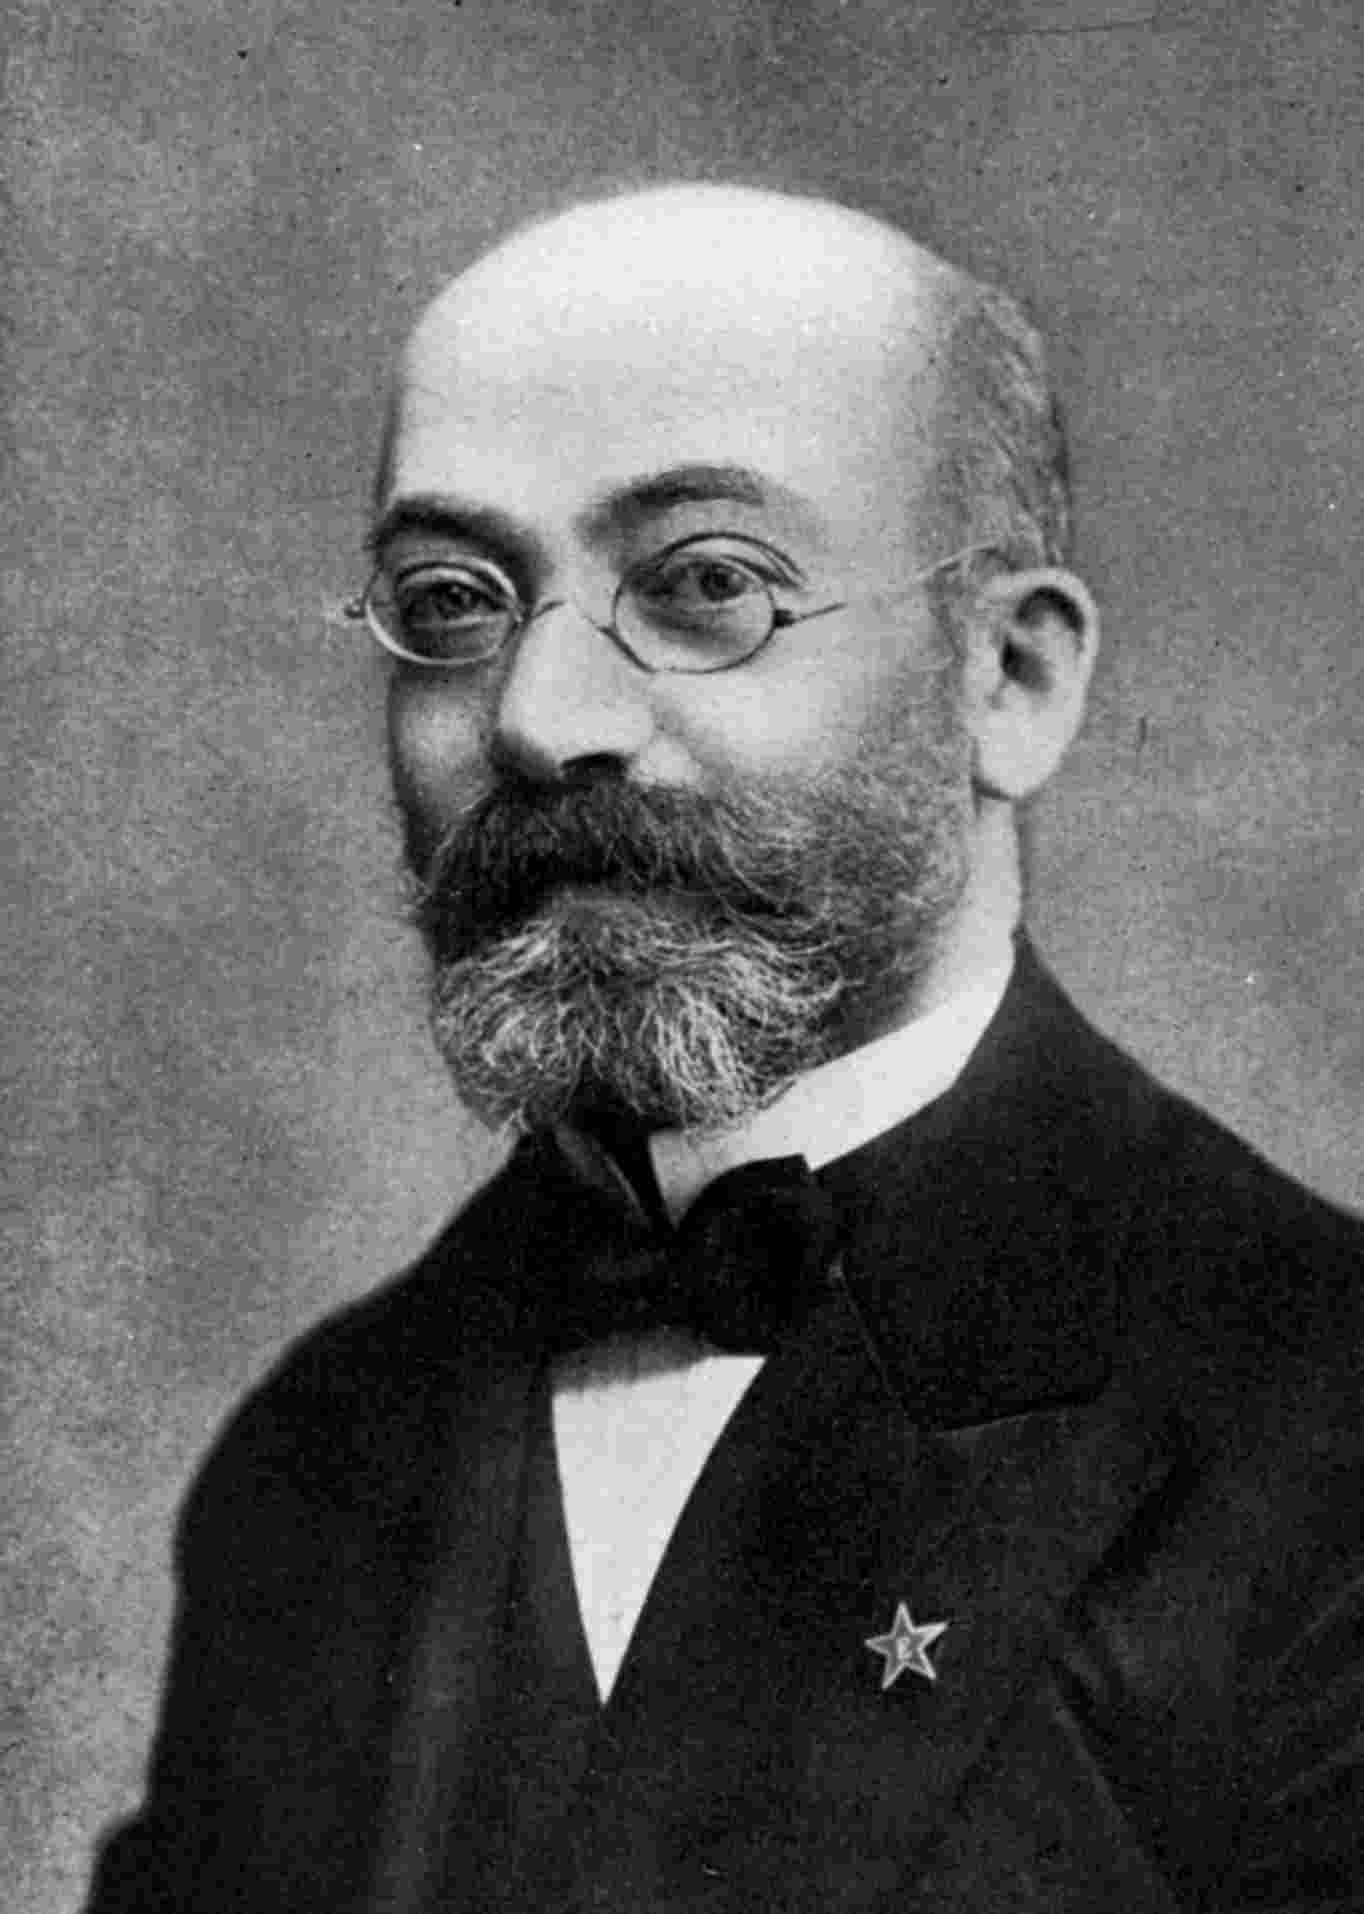
\includegraphics[scale=0.15]{../graphics/Zamenhof}
\end{figure}
\vspace*{0.5cm}
\nicefont
{\LARGE Lazaro Ludoviko ZAMENHOF} \\[1ex]
{\large Aŭtoro de la lingvo «Esperanto»} \\[1ex]
{\small (la 15-a de Decembro 1859 --- la 14-a de Aprilo 1917)}
 \vspace*{\stretch{1}}
\end{center}
\newpage
}

% Ligiloj, kaj ilia koloro 
%
\usepackage{color}
\definecolor{verda_ligilo}{rgb}{0,0.5,0}
\usepackage[colorlinks,linkcolor=verda_ligilo]{hyperref}
\usepackage{bookmark}
